
\chapter{Assessing User's Perceptions of Blockchain}

We highlighted the potential applications of blockchains, as well as some research that has already been conducted until now. It starts to be clearer that blockchain technology has far more potential, than exclusively as a means to register transactions of decentralized cryptocurrencies. Nonetheless, to the authors' knowledge, there's few or nonexistent research in regards as to how humans perceive blockchain technology. Although there's increasing research regarding using blockchain technology, for solving security, privacy and access control issues, in an increasingly decentralized and complex society, there's little research over how humans perceive that disruption.
  
Important factors for the adoption of a given technology or technique are the perceived relevance, complexity and suitability for the task at hand: \emph{How can we understand how humans will embrace the blockchain disruption if we don't understand how they perceive the underlying technology?} It is a fact that end-users are increasing their blockchain-based cryptocurrencies adoption, along with the market value increase of several cryptocurrencies. Yet, the understanding of how humans embrace these new decentralized applications built on top of blockchains (not only Bitcoin's blockchain but other sorts of blockchains as well) is still unknown. This is an enormous gap in our knowledge, in the sense that we have been funding millions of dollars for startups with the promise of building technologies on top of blockchain technologies, yet we cannot even grasp how humans will react to that disruption. If human perspective is not accounted in the design of new blockchain applications, they would be very likely to fail.

Furthermore, we have yet to understand how users perceive blockchain's complexity or inherent security, if they understand the technology or the concepts or whether such a technology would appeal to them. Do humans perceive blockchain has having the same potential as the academic literature, described before, makes it seem? Do users perceive blockchains as viable solutions to the problems we are, collectively, aiming to solve? These questions are our starting point for the forthcoming controlled experiment.

The aim of our research is to start filling in that gap by studying how humans perceive BlockChain technology, regarding its security and complexity. This has been done by conducting a study, based on an online questionnaire, that attempts to get insights on these matters. In this study we focus on two research questions:
  
\begin{itemize}
    \item \textbf{RQ1} - What is the perceived level of security in BlockChain-based solutions, compared to other solutions?
    \item \textbf{RQ2} - What is the perceived complexity introduced by BlockChain-based solutions?
\end{itemize}

The aims of the study are two-fold: \emph{(i)} filling a gap in current knowledge regarding BlockChain-based technologies, namely the human perception, and \emph{(ii)} focus on the perceived value of BlockChain-based solutions for the challenge of educational certificate issuance, sharing and validation. Specifically, we aim at understanding how humans perceive BlockChain-based solutions, in the context of educational certificates, in terms of security and complexity. The online questionnaire was conducted with 46 respondents.
  
\section{Study Design}

In the previous section, the importance of educational certificates to validate the achievements and capabilities that a specific individual possesses is described. It is also described how, with the growing trend in MOOC-based education, issuing, storing, sharing and validating educational certificates is starting to become and interesting challenge to overcome. Moreover, we have also described how some research has been attempting to solve this challenge by using blockchain technologies. At the same time, we have reviewed how research into security, privacy and access control has, too, been increasingly studying usage of blockchain technologies for some challenges of those fields. With that, we have motivated how a lack of research over human perception of the blockchain technologies can pose further challenges into the adoption and usage of blockchain technologies, in deeper research.
  
\subsection{Business Actors and Interactions}

An initial set of business actors was established for the processes we described in the questionnaire: \textit{Student}, \textit{Educational Institution} and \textit{Recruiter}. In this situation we are using a third-party actor - \textit{Recruiter} - for the specific use case of trying to share a digital certificate with a recruiter for the purpose of, for example, validating that a \textit{Student} has the educational background its claims. The \textit{Student} is the requester of the certificate that needs to be issued, or is going to be shared. It is the individual that is the rightful owner of the certificate and should determine who has access to it. The \textit{Educational Institution} is the one that is able to generate new certificates, requested by the Requester. It has the capability to validate all requests as well as issue the certificates. Finally, the \textit{Recruiter} serves the purpose of being an individual, with which a certificate might be shared and might want to validate its authenticity. 

\begin{figure}[htb]
    \centering
    \begin{subfigure}[b]{0.3\textwidth}
        \centering
        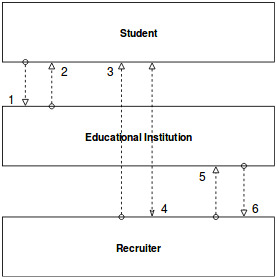
\includegraphics[width=0.8\textwidth]{Scenario1}
        \caption{Interactions in Scenario 1}
        \label{fig: Scenario1}
    \end{subfigure}
    %
    \begin{subfigure}[b]{0.3\textwidth}
        \centering
        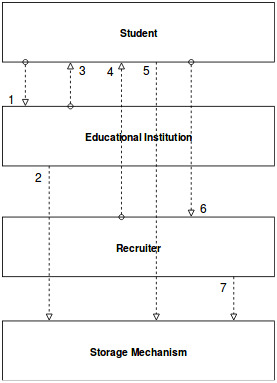
\includegraphics[width=0.8\textwidth]{Scenario2}
        \caption{Interactions in Scenario 2} 
        \label{fig: Scenario2}
    \end{subfigure}
    %
    \begin{subfigure}[b]{0.3\textwidth}
        \centering
        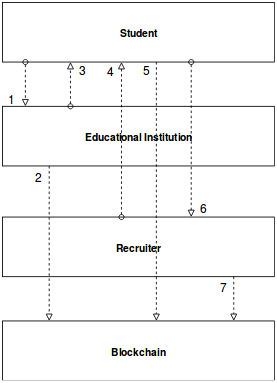
\includegraphics[width=0.8\textwidth]{Scenario3}
        \caption{Interactions in Scenario 3} 
        \label{fig: Scenario3}
    \end{subfigure}
    
    \caption{Interactions presented to Respondents.}
\end{figure}

\subsection{Methodology}
  
This section discusses the methodology used throughout the questionnaire. Firstly, the design of the questionnaire and its contents is discussed, and afterwards, the presentation and distribution is explained.

The questionnaire was designed to target professionals in multiple industries with different backgrounds and knowledge levels. It had 28 questions, of which 21 were mandatory questions and 7 optional. There were 5 sections on the questionnaire: \textit{Introduction}, \textit{Background}, \textit{Exercise 1}, \textit{Exercise 2} and \textit{Final Survey}. There was no time limit nor were the respondents offered with any incentives. Participation was completely voluntary.
%
\textit{Introduction} explained the research objectives, the context in which it was inserted and it stated that all answers were anonymous and would only be used, and shared for academic purposes. 
%
\textit{Background} had four questions, with the aim of assessing respondents' professional and academic background, as well as their perceived knowledge of specific technologies and concepts. Those questions were:
%
\emph{(i)} Do you have any academic or professional background related with Information Security? 
\emph{(ii)} Which industry best fits with your professional experience? 
\emph{(iii)} Which professional role best fits your experience? 
and \emph{(iv)} How do you classify your knowledge of the following concepts?
%
In \textit{Exercise 1} and \textit{Exercise 2}, respondents were asked to answer specific questions. In \textit{Exercise 1} there were two separate scenarios to analyze. In \textit{Exercise 2} there was only one scenario to analyze. In each scenario, there was a simple \gls{bpmn} \cite{BPMN} model followed by a description of the interactions between the actors. All three scenarios had exactly the same 7 questions: 
%
\emph{(i)} Which level of security do you perceive in each interaction? 
\emph{(ii)} Which level of security do you perceive in the entire process? 
\emph{(iii)} What could make it more secure? 
\emph{(iv)} Select any interactions you perceive as allowing unauthorized access to information being shared, 
\emph{(v)} If you were a Student, what would be your willingness to share information, in this context, with a Recruiter? 
\emph{(vi)} If you were a Student, what would be your confidence that the information you share is secure and no one, except the Recruiter, will access it? 
and \emph{(vii)} Which level of complexity do you perceive in each interaction?

The three scenarios the respondents had to analyze described: 
\emph{(i)} a typical scenario of issuing, sharing and validating an educational certificate, \emph{(ii)} a typical scenario, using an undisclosed storage mechanism, such as a database, with added access control functionality, and \emph{(iii)} a typical scenario, using a BlockChain, with added access control functionality.

The respondents were never asked to compare any scenario, but only asked to answer the same questions for each scenario.

In the last section, \textit{Final Survey}, the respondents were asked two additional questions and a placeholder for some comments, if necessary: \emph{(i)} Do you think any of the previous 3 scenarios was more secure than the others? and \emph{(ii)} Do you believe knowledge of Information Security, its applications and concepts, is at an adequate level in your professional environment?


Out of the 7 questions, 5 were based on Likert scales from 0 to 4, where 0 was the lowest possible value and 4 the highest possible value. 1 question was open-ended question and 1 was a checkbox question. These questions, from each scenario, 21 questions in total, were the core of our study.

Two versions were made out of the same questionnaire. The first version had the following sequence: Typical scenario, Storage Mechanism scenario and BlockChain scenario. The second version had the following sequence: Storage Mechanism scenario, Typical scenario and BlockChain scenario. Respondents were redirected to one of the versions without knowing which version and without knowing that several versions existed. The aim of this separation was to try and mitigate the learning effects that answering a questionnaire on a given sequence can generate.

The questionnaire was pretested with 1 respondent to validate previous problems before distribution and, after necessary corrections, was distributed. Distribution took place, initially, over email to a controlled group of 5 people to ensure the randomization system was working properly and that no errors occurred with submission, this was in order mitigate further problems before sending the questionnaire to more people. After that, it was sent, via email, to a group of 50 people, mainly professionals. That group grew to about 150 people. After that, the questionnaire was also posted on HackerNews, as a LinkedIn post and in Reddit, in /r/Assistance and /r/SampleSize. The questionnaire was open for answer from May 9, 2018, until May 20, 2018. Overall, we were able to reach 82 participants, of which 46 answered the questionnaire completely.

\section{Results}

This section presents the results of the questionnaire conducted and discusses some potential implications, tendencies and outcomes that can be concluded. We have analyzed both versions of the questionnaire separately, \textit{Version 1} and \textit{Version 2}, and performed a combined analysis, with both versions' data sets. This section is structured in direct relation to the research questions outlined, in Section 1, by looking at the data that relates to each of them.
  
As described previously, 46 respondents answered the questionnaire, with 24 respondents answering \textit{Version 1} (52\%) and 22 respondents answering \textit{Version 2} (48\%). There was a balance between respondents with backgrounds related to Information Security - with 52\% of the respondents saying they do have a background related to Information Security. Nonetheless, in \textit{Version 1}, 62.5\% of the respondents said they did not have a background related to Information Security. Industries and roles (see Table \ref{tab: industry} and table \ref{tab: roles}) tended to be in the area of Software Development.

For simplicity of our analysis, we have corrected the switch made between \textit{Version 1} and \textit{Version 2}, when reporting the results, in order to allow a direct comparison between both data sets, instead of having to mentally compare them.

\begin{table}[htb]
    \centering
    \caption{Industry Frequency}
    \label{tab: industry}
    \begin{tabular}{l|cc|c}
    \hline \bf Industry & \bf Version 1 & \bf Version 2  & \bf Both \\ \hline
    Consultancy   & 5 & 1  & 6  \\
    Telecom.     & 1 & 1  & 2  \\
    Software Dev. & 9 & 15 & 24 \\
    R\&D          & 1 & 1  & 2  \\
    Academic      & 4 & 3  & 7  \\
    Other         & 2 & 1  & 3  \\
    N.A.          & 1 & 0  & 1  \\
    Health        & 1 & 0  & 1  \\
    \hline
    \end{tabular}
\end{table}

\begin{table}[htb]
    \centering
    \caption{Role Frequency}
    \label{tab: roles}
    \begin{tabular}{l|cc|c}
    \hline \bf Role & \bf Version 1 & \bf Version 2  & \bf Both \\ \hline
    Software Dev.    & 13 & 12  & 25  \\
    Researcher       & 2 & 2  & 4  \\
    Professor        & 1 & 15 & 24 \\
    Business Manager & 5 & 1  & 6  \\
    Project Manager  & 1 & 4  & 5  \\
    Other            & 1 & 1  & 2  \\
    N.A.             & 1 & 0  & 1  \\
    \hline
    \end{tabular}
\end{table}

Respondent's perceived knowledge of specific concepts, from 0 (lowest) to 4 (highest), slightly varied between versions, with \textit{Version 2} presenting a more knowledgeable set of respondents, in most concepts (see Table \ref{tab: knowledge}), with the concepts being: \emph{(i)} Access Control; \emph{(ii)} Encryption; \emph{(iiii)} BlockChain; \emph{(iv)} Data Integrity; \emph{(v)} Malware; \emph{(vi)} Phishing; \emph{(vii)} Data Confidentiality; \emph{(viii)} BPMN; \emph{(ix)} Data Storage; \emph{(x)} Unauthorized Access.

\begin{table}[htb]
    \centering
    \caption{Reported Knowledge Using the Scale 0 (Lowest) to 4 (Highest)}
    \label{tab: knowledge}
    \begin{tabular}{c|cccc|cc}
    \hline 
    \bf Concept & \multicolumn{2}{c}{\bf Version 1} & \multicolumn{2}{c}{\bf Version 2} \vrule & \multicolumn{2}{c}{\bf Both} \\
    \hline
     & $\tilde{x}$ & $\sigma_{x}$ & $\tilde{x}$ & $\sigma_{x}$ & $\tilde{x}$ & $\sigma_{x}$ \\
    \hline
    1 & 1.92 & 0.97 & 2.36 & 1.18 & 2.13 & 1.09 \\
    2 & 1.67 & 1.05 & 2.14 & 1.13 & 1.89 & 1.10 \\
    3 & 1.33 & 0.87 & 1.05 & 0.84 & 1.20 & 0.86 \\
    4 & 1.83 & 1.09 & 2.14 & 1.21 & 1.98 & 1.15 \\
    5 & 1.71 & 0.91 & 1.82 & 0.96 & 1.76 & 0.92 \\
    6 & 1.96 & 0.91 & 2.14 & 0.94 & 2.04 & 0.92 \\
    7 & 2.46 & 1.02 & 2.46 & 1.01 & 2.46 & 1.01 \\
    8 & 0.83 & 1.01 & 1.36 & 1.36 & 1.09 & 1.21 \\
    9 & 2.29 & 1.00 & 2.36 & 1.33 & 2.32 & 1.16 \\
    10 & 2.00 & 1.02 & 2.09 & 1.27 & 2.04 & 1.13 \\
    \hline
    \end{tabular}
\end{table}

Regarding our background results, we can conclude that our sample tends towards the Software Development area, followed by professionals from Academia. This means that our sample is subject to having more knowledge on general technology topics, than a more mixed sample would. \textit{Version 1} respondents reported a below-average knowledge of the presented concepts, with a lower standard deviation, while \textit{Version 2} respondents reported a higher than average knowledge of the presented concepts, with a less concentrated set of answers. All coefficients of variation, in the compound analysis, are lower than 1 (between \textit{cv = 0.41} and \textit{cv = 0.72}), except for BPMN (\textit{cv = 1.11}). The same happens for each separate version, with different boundaries.

\subsection{RQ1}

\begin{quote}
\textit{What is the perceived level of security in BlockChain-based solutions, compared to other solutions?}
\end{quote}

To answer this question, we took special attention to questions 1, 2 and 4 of each of the scenarios. In questions 1 and 2, respondents were asked to evaluate the perceived security of a given scenario. The evaluations were for the process in its entirety and for each interaction in the scenario. Question 4 asked respondents to select the interactions they perceived as allowing unauthorized questions. We have also taken in consideration the answers given in the final question, in which respondents were forced to choose which scenario was the most secure.

Starting from the last question, an overwhelming majority of the respondents answered that they perceived the scenario using BlockChain to be the most secure (see Table \ref{tab: mostSecure}) - when forced to choose.

\begin{table}[htb]
    \centering
    \caption{Most Secure Scenario (Total Amount of Responses)}
    \label{tab: mostSecure}
    \begin{tabular}{l|ccc}
    \hline \bf Answer & \bf Version 1 & \bf Version 2  & \bf Both \\ \hline
    None       & 1  & 1  & 2  \\
    Scenario 1 & 1  & 4  & 5  \\
    Scenario 2 & 3  & 3  & 6 \\
    Scenario 3 & 19 & 14 & 33  \\
    \hline
    \end{tabular}
\end{table}

This suggests that there's a tendency to believe that BlockChain-based solutions are perceived as being more secure than other solutions. The fact that users were forced to choose one or none of the scenarios makes it more clear that, although we cannot claim any justification for it, respondents had a tendency to claim that BlockChain-based solutions are more secure than other solutions. Even more interesting is that not only did respondents chose BlockChain-based solutions against the typical scenario but the same occurred for the scenario that used a basic Storage Mechanism, instead of Blockchain.

For the first question, which asked for the perceived level of security in each scenario (see Table \ref{tab: perceivedSecurity}), we witnessed similar results. We witness the same effect, in \textit{Version 2}, as we had previously, although the data is more spread (\textit{$\sigma_{x}$ = 1.23}).

\begin{table}[htb]
    \centering
    \caption{Perceived Security / Scenario Using the Scale 0 (Lowest) to 4 (Highest)}
    \label{tab: perceivedSecurity}
    \begin{tabular}{c|cccc|cc}
    \hline 
    Scenario & \multicolumn{2}{c}{\bf Version 1} & \multicolumn{2}{c}{\bf Version 2} \vrule & \multicolumn{2}{c}{\bf Both} \\
    \hline
     & $\tilde{x}$ & $\sigma_{x}$ & $\tilde{x}$ & $\sigma_{x}$ & $\tilde{x}$ & $\sigma_{x}$ \\
    \hline
    1 & 2.13 & 0.99 & 2.50 & 1.23 & 2.30 & 1.11 \\
    2 & 2.83 & 0.96 & 2.36 & 0.95 & 2.61 & 0.98 \\
    3 & 3.00 & 0.89 & 2.91 & 0.87 & 2.96 & 0.87 \\
    \hline
    \end{tabular}
\end{table}

We can understand, by studying the coefficients of variation (Version 1: Scenario 1 (\textit{cv = 0.47}), Scenario 2 (\textit{cv = 0.34}), Scenario 3 (\textit{cv = 0.29}); Version 2: Scenario 1 (\textit{cv = 0.48}), Scenario 2 (\textit{cv = 0.40}), Scenario 3 (\textit{cv = 0.30}) that respondents' answers became more concentrated when it comes to BlockChain-based solutions (Scenario 3), while being more dispersed in Storage Mechanism (Scenario 2) and even more in the typical process (Scenario 1). This further reinforces the appearing tendency.

By studying the results of the evaluation by interaction, in each scenario, and with the scenario as a whole, the data is less clear than previous answers. Results, seen in Table \ref{tab: perceivedInteractionSecurity}, have shown an increase in the dispersion of the data which impacts mean-based analysis. It is interesting that, contrary to what had happened when asked about the security of the entire process, in this case, in \textit{Version 1}, we cannot see a major difference between the results of Scenario 2 and Scenario 3. Nonetheless, we still see the same patterns as in the previous results, in \textit{Version 2} and when considering the data sets combined. 

\begin{table}[htb]
    \centering
    \caption{Perceived Interaction Security / Scenario Using the Scale 0 (Lowest) to 4 (Highest)}
    \label{tab: perceivedInteractionSecurity}
    \begin{tabular}{c|cccc|cc}
    \hline 
    Scenario & \multicolumn{2}{c}{\bf Version 1} & \multicolumn{2}{c}{\bf Version 2} \vrule & \multicolumn{2}{c}{\bf Both} \\
    \hline
     & $\tilde{x}$ & $\sigma_{x}$ & $\tilde{x}$ & $\sigma_{x}$ & $\tilde{x}$ & $\sigma_{x}$ \\
    \hline
    1 & 2.26 & 1.30 & 2.58 & 1.21 & 2.42 & 1.26 \\
    2 & 2.71 & 1.13 & 2.27 & 1.43 & 2.50 & 1.30 \\
    3 & 2.68 & 1.12 & 2.72 & 1.19 & 2.70 & 1.15 \\
    \hline
    \end{tabular}
\end{table}

In Figure \ref{fig: perceivedInteractionSecurityOne} we expose the data used to generate Table \ref{tab: perceivedInteractionSecurity}'s \textit{Version 1}, as line charts, in which the data sets for each scenario have been run through a probability density function. This allows us to see that the mean, for Scenario 2, is highly influenced by more skewed distributions and, at the same time, it confirms, visually, the data about the process as a whole. Scenario 3 is visually more secure and concentrated - the interactions perceived as more secure, individually.

\begin{figure}[htb]
    \centering
    \begin{subfigure}[b]{0.49\textwidth}
        \centering
        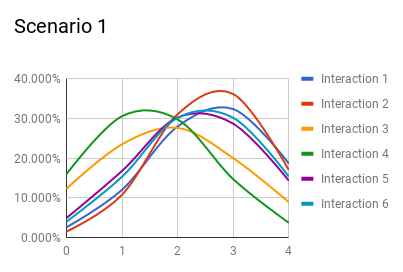
\includegraphics[width=\linewidth]{V1-S1-Security.png}
    \end{subfigure}
    %
    \begin{subfigure}[b]{0.49\textwidth}
        \centering
        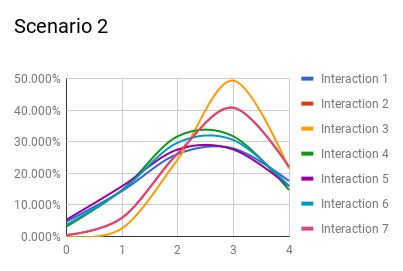
\includegraphics[width=\linewidth]{V1-S2-Security.png}
    \end{subfigure}
    %
    \hfill
    \begin{subfigure}[b]{0.49\textwidth}
        \centering
         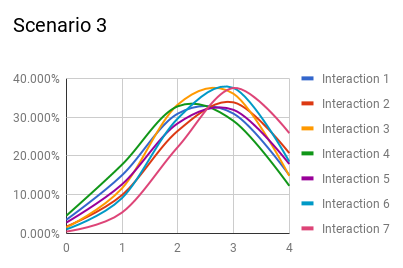
\includegraphics[width=\linewidth]{V1-S3-Security.png}
    \end{subfigure}
    
    \caption{Probability Density of Perceived Interaction Security (Version 1)}
    \label{fig: perceivedInteractionSecurityOne}   
\end{figure}

At the same time, in Figure \ref{fig: perceivedInteractionSecurityTwo} we expose the data used to generate Table \ref{tab: perceivedInteractionSecurity}'s \textit{Version 2}. The visualizations closely resembles the one presented in Figure \ref{fig: perceivedInteractionSecurityOne}. This is relevant due to the fact that the aggregate numbers, shown in Table \ref{tab: perceivedInteractionSecurity}, only allow us to have a high-level understanding, of the respondents' perception. The visualizations help understand that, even in more detail, the data is similarly distributed, although, somehow skewed to the left, in Scenario 1, and skewed to the right.

\begin{figure}[htb]
    \centering
    \begin{subfigure}[b]{0.49\textwidth}
        \centering
        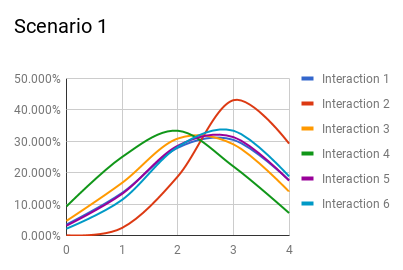
\includegraphics[width=\linewidth]{V2-S1-Security.png}
    \end{subfigure}
    %
    \begin{subfigure}[b]{0.49\textwidth}
        \centering
        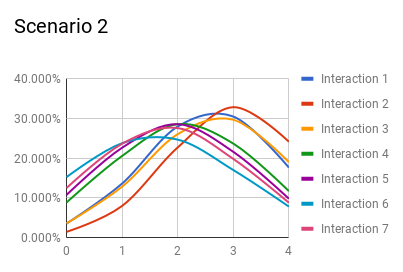
\includegraphics[width=\linewidth]{V2-S2-Security.png}
    \end{subfigure}
    %
    \hfill
    \begin{subfigure}[b]{0.49\textwidth}
        \centering
        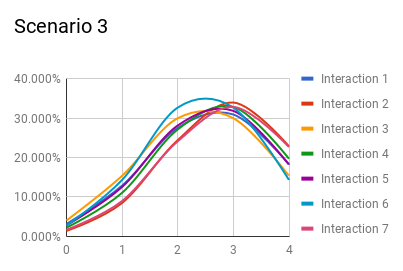
\includegraphics[width=\linewidth]{V2-S3-Security.png}
    \end{subfigure}
    
    \caption{Probability Density of Perceived Interaction Security (Version 2)}
    \label{fig: perceivedInteractionSecurityTwo}   
\end{figure}

\subsection{RQ2}

\begin{quote}
\textit{What is the perceived complexity introduced by BlockChain-based solutions?}
\end{quote}

\begin{table}[htb]
    \centering
    \caption{Perceived Complexity / Scenario Using the Scale 0 (Lowest) to 4 (Highest)}
    \label{tab: perceivedComplexity}
    \begin{tabular}{c|cccc|cc}
    \hline 
    Scenario & \multicolumn{2}{c}{\bf Version 1} & \multicolumn{2}{c}{\bf Version 2} \vrule & \multicolumn{2}{c}{\bf Both} \\
    \hline
     & $\tilde{x}$ & $\sigma_{x}$ & $\tilde{x}$ & $\sigma_{x}$ & $\tilde{x}$ & $\sigma_{x}$ \\
    \hline
    1 & 1.56 & 1.51 & 1.47 & 1.13 & 1.51 & 1.14 \\
    2 & 1.96 & 1.21 & 1.71 & 1.25 & 1.82 & 1.23 \\
    3 & 2.25 & 1.26 & 1.97 & 2.00 & 2.12 & 1.24 \\
    \hline
    \end{tabular}
\end{table}

For this question, we have analyzed the answers to question 7 of each scenario, which asked respondents to grade each interaction they were shown, in terms of its complexity. We present the mean for all interactions' evaluation and also the standard deviation, per scenario (see Table \ref{tab: perceivedSecurity}). The results show that there's an increase in the perceived complexity of BlockChain-based solutions. In this case, contrary to what happened with the previous research question, we do not see a pronounced learning bias as, regardless of the order of the questions, the tendency remained the same - and the compound analysis reflected that situation. It is also interesting to notice that, when asked about the concept of complexity, the dispersion of data increases, specially when compared to the concept of security.

Finally, respondents also perceived that sharing the certificate, under a BlockChain-based solution, had fewer interactions with the possibility of allowing unauthorized access to data, than with the typical purpose. The same is true for BlockChain-based solutions over the Storage Mechanism.

\begin{figure}[htb]
    \centering
    \begin{subfigure}[b]{0.49\textwidth}
        \centering
        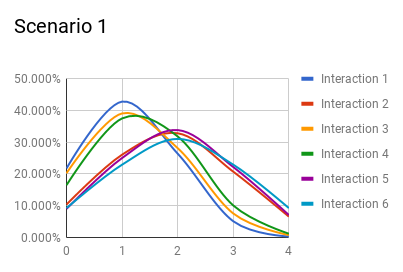
\includegraphics[width=\linewidth]{V1-S1-Complexity.png}
    \end{subfigure}
    %
    \begin{subfigure}[b]{0.49\textwidth}
        \centering
        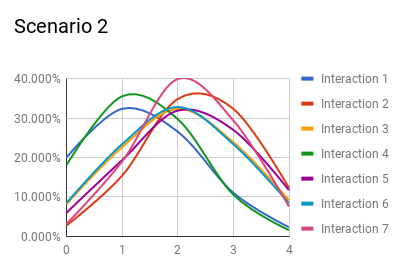
\includegraphics[width=\linewidth]{V1-S2-Complexity.png}
    \end{subfigure}
    %
    \hfill
    \begin{subfigure}[b]{0.49\textwidth}
        \centering
        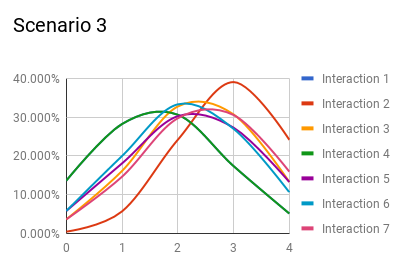
\includegraphics[width=\linewidth]{V1-S3-Complexity.png}
    \end{subfigure}
    
    \caption{Probability Density of Perceived Interaction Complexity (Version 1)}
    \label{fig: perceivedInteractionComplexityOne}    
\end{figure}

\begin{figure}[htb]
    \centering
    \begin{subfigure}[b]{0.49\textwidth}
        \centering
        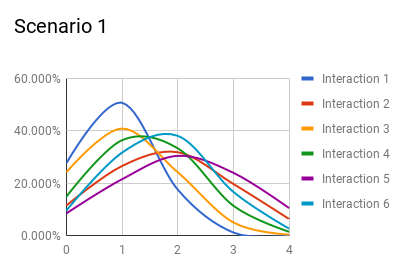
\includegraphics[width=\linewidth]{V2-S1-Complexity.png}
    \end{subfigure}
    %
    \begin{subfigure}[b]{0.49\textwidth}
        \centering
        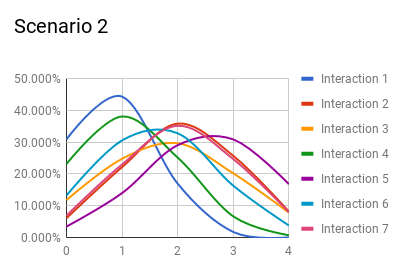
\includegraphics[width=\linewidth]{V2-S2-Complexity.png}
    \end{subfigure}
    %
    \hfill
    \begin{subfigure}[b]{0.49\textwidth}
        \centering
        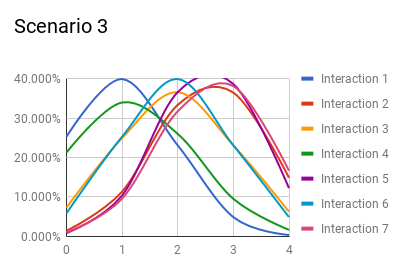
\includegraphics[width=\linewidth]{V2-S3-Complexity.png}
    \end{subfigure}
    
    \caption{Probability Density of Perceived Interaction Complexity (Version 2)}
    \label{fig: perceivedInteractionComplexityTwo}   
\end{figure}

Figure \ref{fig: perceivedInteractionComplexityOne} and Figure \ref{fig: perceivedInteractionComplexityTwo} allow us to perform the same visual comparison, such as in the previous section. What we see indicates what has been shown in the high-level picture, both in terms of mean and standard deviation. For example, in the BlockChain-based solutions (Scenario 3), in \textit{Version 2} , the data is very spread when compared inter-interaction but it seems to be much more concentrated for each interaction than in \textit{Version 1}.
  
\section{Discussion}

\subsection{Limitations}

This section describes the limitations found with the present study. The objective is to address these shortcomings in future studies. 
  
Firstly, it is important to note that this is a small sample, less than 50 respondents. This situation can give rise to erroneous results due to bias sampling. At the same time, although we have some diversity, we would like to decrease the majority of one specific field of the others and gather a more diverse set of respondents. This limitation can be overcome by reproducing the questionnaire on larger, more diverse samples. 
  
Secondly, we would also like to leave a note regarding the possibility of learning bias. Although we have shuffled our scenarios, we have only done that with 2 out of the 3 scenarios. In order to be able to get more conclusive data, it would be important to perform different studies where more shuffling was involved, particularly with anything involving blockchain - which we have kept in the last position, in both versions. 
  
Finally, the platform used for the questionnaire had two limitations: a back button - which allowed respondents to rewrite their answers - and the impossibility to present the images of the interactions along with the questions - which might increase the confusion in respondents, by having to memorize the images.
  
\section{Summary}

The research presented in this paper presents an overlap between several areas of research: Information Security, BlockChain, Educational Certificates and Human Perception. We sought to explore how those interact by conducting an online questionnaire followed by a study that would shed some light over how humans perceive BlockChain technology, in terms of security and complexity, in an Educational Certificate use case. The results have indicated a tendency for humans to perceive BlockChain technology as more secure but, alas, more complex too - at least in this particular domain. Future research should be focused on resolving the limitations pointed out in this paper and, at the same time, focus on trying to explore the correlation and causal variables that produce these perceptions. This research is a starting point to better understand how humans perceive BlockChain technology.